
\section*{Solutions to Exercises From Section 1}

\begin{solution}\label{sol:1.1}\ref{ex:1.1}
\begin{enumerate}
    \item $\{ 5x-1:x\in\Z \}=\{ \dots,-6,-1,4,9,\dots \}$.
    \item $\{ 3x+2:x\in\Z \}=\{ \dots,-1,2,5,8,\dots \}$. 
    \item $\{ x\in\Z: -2\le x\le 7\}=\{ -2,-1,0,1,2,3,4,5,6,7 \}$. 
    \item $\{ x\in\N:-2 < x \le 7 \}=\{ 0,1,2,3,4,5,6,7 \}$.
    \item $\{ x\in\R:x^2=3 \}=\{ -\sqrt 3, \sqrt 3 \}$.
    \item $\{ x\in\R:x^2=9 \}=\{ -3,3 \}$.
    \item $\{ x\in\R:x^2+5x=-6 \}=\{ -2,-3 \}$.
    \item $\{ x\in\R:x^3+5x^2=-6x \}=\{ -3,-2,0 \}$.
    \item $\{ x\in\R:\sin\pi x=0 \}=\Z$.
    \item $\{ x\in\R:\cos x=1 \}=\{ 2n\pi:n\in\Z \}$.
    \item $\{ x\in\Z:\lvert x \rvert<5 \}=\{ -4,-3,-2,-1,0,1,2,3,4 \}$.
    \item $\{ x\in\Z: \lvert 2x \rvert<5 \}=\{ -2,-1,0,1,2 \}$.
    \item $\{ x\in\Z:\lvert 6x \rvert<5 \}=\{ 0 \}$.
    \item $\{ 5x:x\in\Z,\lvert 2x \rvert\le8 \}=\{ -20,-15,-10,-5,0,5,10,15,20 \}$.
    \item $\{ 5a+2b:a,b\in\Z \}=\Z$.
    \item $\{ 6a+2b:a,b\in\Z \}=2\Z$.
\end{enumerate}

\end{solution}

\begin{solution}\label{sol:1.2}\ref{ex:1.2}
    \emph{Tip:} Some problems might look intimidating but in general, the easiest way to complete a problem like this, would be to consider the following three steps. 
    \begin{enumerate}
        \item [1] Is there common denominator? 
        \item [2] Is there a constant that can be factored out? 
        \item [3] What remains and how can this be generalised? 
    \end{enumerate}
    With those tips in mind, we proceed to the solutions. 
    \begin{enumerate}
        \item[17] $\{ 2,4,8,16,32,64 \}=\{ 2^x:x\in\N \}$
        \item[18] $\{ 0,4,16,36,64,100,\dots \}=\{ x^2:x\in\N,2\mid x \}$.
        \item[19] $\{ \dots,-6,-3,0,3,6,9,12,15,\dots \}=\{ 3x:x\in\Z \}$.
        \item[20] $\{ \dots,-8,-3,2,7,12,17,\dots \}=\{ 5x+2:x\in\Z \}$.
        \item[21] $\{ 0,1,4,9,16,25,36,\dots \}=\{ x^{2}:x\in\N\}$
        \item[22] $\{ 3,6,11,18,27,38,\dots \}=\{x^2+2:x\in\Z^{+}\}$
        \item[23] $\{ 3,4,5,6,7,8 \}=\{ x\in\N: 3\le x \le 8 \}$
        \item[24] $\{ -4,-3,-2,-1,0,1,2 \}=\{ x\in\Z:-4\le x \le 2 \}$
        \item[25] $\{ \dots,\frac{1}{8},\frac{1}{4},\frac{1}{2},1,2,4,8,\dots \}=\{x\in\Z: 2^{-x} \}$  
        \item[26] $\{ \dots,\frac{1}{27},\frac{1}{9},\frac{1}{3},1,3,9,27 \}=\{ 3^{-x}:x\in\Z \}$
        \item[27] $\{ \dots,-\pi,-\frac{\pi}{2},0,\frac{\pi}{2},\pi,\frac{3\pi}{2},2\pi,\frac{5\pi}{2} \}=\{ \frac{n\pi}{2}:n\in\Z \}$
        \item[28] $\{ \dots,-\frac{3}{2},-\frac{3}{4},0,\frac{3}{4},\frac{3}{2},\frac{9}{4},3,\frac{15}{4},\frac{9}{2},\dots \}=\{ \frac{3x}{4}:x\in\Z \}$   
    \end{enumerate}
\end{solution}

\begin{solution}\label{sol:1.3}\ref{ex:1.3}
    \begin{enumerate}
        \item[29] $\lvert \{ \{ 1 \},\{ 2,\{ 3,4 \} \},\varnothing \} \rvert=3$
        \item[30] $\lvert \{ \{ 1,4 \},a,b,\{ \{ 3,4 \} \},\{ \varnothing \} \} \rvert=5$
        \item[31] $\lvert \{ \{ \{ 1 \},\{ 2,\{ 3,4 \} \},\varnothing \} \} \rvert=1$
        \item[32] $\lvert \{ \{ \{ 1,4 \},a,b,\{ \{ 3,4 \} \},\{ \varnothing \} \} \} \rvert=1$  
        \item[33] $\lvert \{ x\in\Z:\lvert x \rvert<10 \} \rvert=19$
        \item[34] $\lvert \{x\in\N:\lvert x \rvert<10 \rvert\}=10$
        \item[35] $\lvert \{ x\in\Z:x^2<10 \} \rvert=7$
        \item[36] $\lvert \{ x\in\N:x^2<10 \} \rvert=4$
        \item[37] $\lvert \{ x\in\N:x^2<0 \} \rvert=0$
        \item[38] $\lvert \{ x\in\N:5x\le20 \} \rvert=5$.   
    \end{enumerate}
\end{solution}

\begin{solution}\label{sol:1.4}\ref{ex:1.4}
    \begin{enumerate}
        \item[39] $\{ (x,y):x\in[1,2],y\in[1,2] \}\Rightarrow$ This would be a solid $1\times 1$ square in $\R^2$ with corners $(1,1),(1,2),(2,1),(2,2)$
        \item[40] $\{ (x,y):x\in[0,1],y\in[1,2] \}\Rightarrow$ This would be a solid $1\times 1$ square in $\R^2$ with corners $(0,1),(0,2),(1,1),(1,2)$.
        \item[41] $\{ (x,y):x\in[-1,1],y=1 \}\Rightarrow$ This would be a line connecting $(-1,1)$ with $(1,1)$. 
        \item[42] $\{ (x,y):x=2,y\in[0,1] \}\Rightarrow$ This would be a line connecting $(2,0),(2,1)$    
        \item[43] $\{ (x,y):\lvert x \rvert=2,y\in[0,1] \}\Rightarrow$ This would be two vertical line segments, that connect $(-2,0)-(-2,1)$ and the other one would be $(2,0)-(2,1)$.
        \item[44] $\{ (x,x^2):x\in\R \}\Rightarrow$ This would be the parabolla $y=x^2$.
        \item[45] $\{ (x,y):x,y\in\R,x^2+y^2=1 \}\Rightarrow$ This would be the unit circle centered at the origin $(0,0)$ with $r=1$
        \item[46] $\{ (x,y):x,y\in\R,x^2+y^2\le 1 \}\Rightarrow$ This would be a disk with $r=1$, centered at $(0,0)$.
        \item[47] $\{ (x,y):x,y\in\R, y\ge x^2-1 \}\Rightarrow$ This would be the region underneath the parabola $y=x^2-1$.
        \item[48] $\{ (x,y):x,y\in\R x>1 \}\Rightarrow$ This would the whole upper right and down left quadrants of the $xy$-plane, or an \emph{open half-plane}, starting from $x=2$. 
        \item[49] $\{ (x,x+y):x\in\R,y\in\Z \}\Rightarrow$ This would be infinitely many parallel lines with slope $1$.
        \item[50] $\{ (x,\frac{x^2}{y})x\in\R,y\in\N\}\Rightarrow$ Division by $0$ is undefined, so we skip those values. Notice that the relation between the first and second coordinate is quadratic, instead of linear. That is to say $v=\frac{u^2}{k}$, so we have a upward-opening parabolas passing through the origin 
        \item[51] $\{ (x,y)\in\R^2:(y-x)(y+x)=0 \}\Rightarrow$ Here we have lines passing through the origin in an X shape. 
        \item[52] $\{ (x,y)\in\R^2:(y-x^2)(y+x^2)=0 \}\Rightarrow$ Lastly, we have two parabolas touching at the origin one opening upwards, one downwards, $y=x^2, y=-x^2$, respectively.
    \end{enumerate}
% --- FIRST PAGE: Items 39 to 45 ---
\begin{figure}[htbp]
    \centering
    \begin{subfigure}[b]{0.3\linewidth}
        \centering
        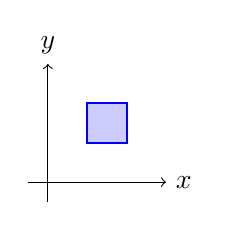
\begin{tikzpicture}[scale=0.5]
            \draw[->] (-0.5,0) -- (3,0) node[right] {$x$};
            \draw[->] (0,-0.5) -- (0,3) node[above] {$y$};
            \fill[blue!20] (1,1) rectangle (2,2);
            \draw[thick, blue] (1,1) rectangle (2,2);
        \end{tikzpicture}
        \caption{Item 39}
    \end{subfigure}\hfill
    \begin{subfigure}[b]{0.3\linewidth}
        \centering
        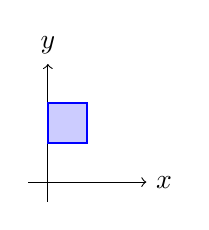
\begin{tikzpicture}[scale=0.5]
            \draw[->] (-0.5,0) -- (2.5,0) node[right] {$x$};
            \draw[->] (0,-0.5) -- (0,3) node[above] {$y$};
            \fill[blue!20] (0,1) rectangle (1,2);
            \draw[thick, blue] (0,1) rectangle (1,2);
        \end{tikzpicture}
        \caption{Item 40}
    \end{subfigure}\hfill
    \begin{subfigure}[b]{0.3\linewidth}
        \centering
        \begin{tikzpicture}[scale=0.5]
            \draw[->] (-2,0) -- (2,0) node[right] {$x$};
            \draw[->] (0,-0.5) -- (0,2) node[above] {$y$};
            \draw[very thick, blue] (-1,1) -- (1,1);
            \filldraw[blue] (-1,1) circle (2pt) (1,1) circle (2pt);
        \end{tikzpicture}
        \caption{Item 41}
    \end{subfigure}

    \vspace{0.5cm}

    \begin{subfigure}[b]{0.3\linewidth}
        \centering
        \begin{tikzpicture}[scale=0.5]
            \draw[->] (-0.5,0) -- (3,0) node[right] {$x$};
            \draw[->] (0,-0.5) -- (0,2) node[above] {$y$};
            \draw[very thick, blue] (2,0) -- (2,1);
            \filldraw[blue] (2,0) circle (2pt) (2,1) circle (2pt);
        \end{tikzpicture}
        \caption{Item 42}
    \end{subfigure}\hfill
    \begin{subfigure}[b]{0.3\linewidth}
        \centering
        \begin{tikzpicture}[scale=0.5]
            \draw[->] (-3,0) -- (3,0) node[right] {$x$};
            \draw[->] (0,-0.5) -- (0,2) node[above] {$y$};
            \draw[very thick, blue] (-2,0) -- (-2,1);
            \draw[very thick, blue] (2,0) -- (2,1);
            \filldraw[blue] (-2,0) circle (2pt) (-2,1) circle (2pt) (2,0) circle (2pt) (2,1) circle (2pt);
        \end{tikzpicture}
        \caption{Item 43}
    \end{subfigure}\hfill
    \begin{subfigure}[b]{0.3\linewidth}
        \centering
        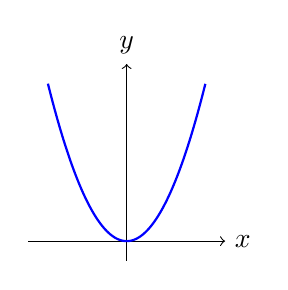
\begin{tikzpicture}[scale=0.5]
            \draw[->] (-2.5,0) -- (2.5,0) node[right] {$x$};
            \draw[->] (0,-0.5) -- (0,4.5) node[above] {$y$};
            \draw[thick, blue, domain=-2:2, samples=100] plot (\x, {\x*\x});
        \end{tikzpicture}
        \caption{Item 44}
    \end{subfigure}

    \vspace{0.5cm}

    \begin{subfigure}[b]{0.3\linewidth}
        \centering
        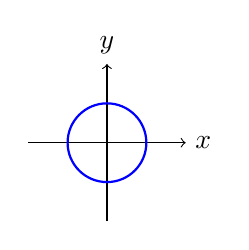
\begin{tikzpicture}[scale=0.5]
            \draw[->] (-2,0) -- (2,0) node[right] {$x$};
            \draw[->] (0,-2) -- (0,2) node[above] {$y$};
            \draw[thick, blue] (0,0) circle (1);
        \end{tikzpicture}
        \caption{Item 45}
    \end{subfigure}
    \caption{Geometric Representations 39--45}\label{fig:geom_part1}
\end{figure}
% --- SECOND PAGE: Items 46 to 52 ---
\begin{figure}[htbp]
    \ContinuedFloat% Keeps the figure numbering the same
    \centering
    \begin{subfigure}[b]{0.3\linewidth}
        \centering
        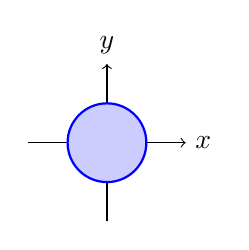
\begin{tikzpicture}[scale=0.5]
            \draw[->] (-2,0) -- (2,0) node[right] {$x$};
            \draw[->] (0,-2) -- (0,2) node[above] {$y$};
            \filldraw[fill=blue!20, draw=blue, thick] (0,0) circle (1);
        \end{tikzpicture}
        \caption{Item 46}
    \end{subfigure}\hfill
    \begin{subfigure}[b]{0.3\linewidth}
        \centering
        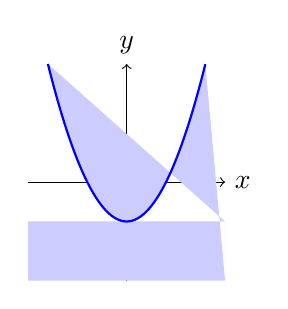
\begin{tikzpicture}[scale=0.5]
            \draw[->] (-2.5,0) -- (2.5,0) node[right] {$x$};
            \draw[->] (0,-2.5) -- (0,3) node[above] {$y$};
            \begin{scope}
                \clip (-2.5,-2.5) rectangle (2.5,3);
                \fill[blue!20] (-2.5,-2.5) rectangle (2.5,-1) -- plot[domain=-2:2, samples=100] (\x, {\x*\x - 1}) -- (2.5,-2.5);
                \draw[thick, blue, domain=-2:2, samples=100] plot (\x, {\x*\x - 1});
            \end{scope}
        \end{tikzpicture}
        \caption{Item 47}
    \end{subfigure}\hfill
    \begin{subfigure}[b]{0.3\linewidth}
        \centering
        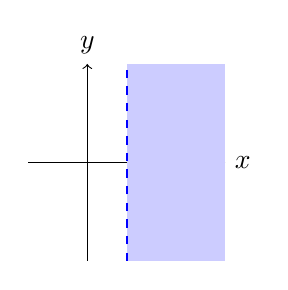
\begin{tikzpicture}[scale=0.5]
            \draw[->] (-1.5,0) -- (3.5,0) node[right] {$x$};
            \draw[->] (0,-2.5) -- (0,2.5) node[above] {$y$};
            \fill[blue!20] (1,-2.5) rectangle (3.5,2.5);
            \draw[dashed, thick, blue] (1,-2.5) -- (1,2.5);
        \end{tikzpicture}
        \caption{Item 48}
    \end{subfigure}

    \vspace{0.5cm}

    \begin{subfigure}[b]{0.3\linewidth}
        \centering
        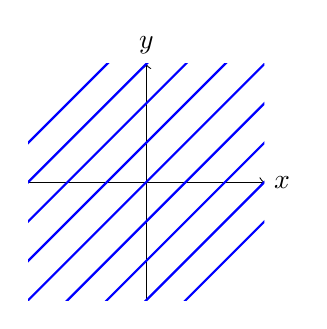
\begin{tikzpicture}[scale=0.5]
            \draw[->] (-3,0) -- (3,0) node[right] {$x$};
            \draw[->] (0,-3) -- (0,3) node[above] {$y$};
            \begin{scope}
                \clip (-3,-3) rectangle (3,3);
                \foreach \k in {-4,-3,...,4} {
                    \draw[thick, blue, domain=-4:4] plot (\x, {\x + \k});
                }
            \end{scope}
        \end{tikzpicture}
        \caption{Item 49}
    \end{subfigure}\hfill
    \begin{subfigure}[b]{0.3\linewidth}
        \centering
        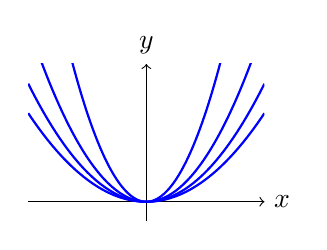
\begin{tikzpicture}[scale=0.5]
            \draw[->] (-3,0) -- (3,0) node[right] {$x$};
            \draw[->] (0,-0.5) -- (0,3.5) node[above] {$y$};
            \begin{scope}
                \clip (-3,-0.5) rectangle (3,3.5);
                \foreach \k in {1,2,3,4} {
                    \draw[thick, blue, domain=-3:3, samples=100] plot (\x, {(\x*\x)/\k});
                }
            \end{scope}
        \end{tikzpicture}
        \caption{Item 50}
    \end{subfigure}\hfill
    \begin{subfigure}[b]{0.3\linewidth}
        \centering
        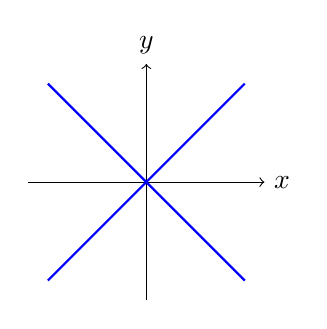
\begin{tikzpicture}[scale=0.5]
            \draw[->] (-3,0) -- (3,0) node[right] {$x$};
            \draw[->] (0,-3) -- (0,3) node[above] {$y$};
            \draw[thick, blue] (-2.5,-2.5) -- (2.5,2.5);
            \draw[thick, blue] (-2.5,2.5) -- (2.5,-2.5);
        \end{tikzpicture}
        \caption{Item 51}
    \end{subfigure}

    \vspace{0.5cm}

    \begin{subfigure}[b]{0.3\linewidth}
        \centering
        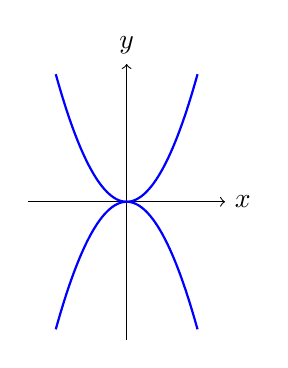
\begin{tikzpicture}[scale=0.5]
            \draw[->] (-2.5,0) -- (2.5,0) node[right] {$x$};
            \draw[->] (0,-3.5) -- (0,3.5) node[above] {$y$};
            \draw[thick, blue, domain=-1.8:1.8, samples=100] plot (\x, {\x*\x});
            \draw[thick, blue, domain=-1.8:1.8, samples=100] plot (\x, {-\x*\x});
        \end{tikzpicture}
        \caption{Item 52}
    \end{subfigure}

    \caption{Geometric Representations 46--52 (Continued)}\label{fig:geom_part2}
\end{figure}
\end{solution}